\documentclass[a4paper,12pt]{article}
\usepackage[utf8]{inputenc}
\usepackage[T1]{fontenc}

\usepackage[left=1.5cm, right=1.5cm, top=2cm, bottom=2cm, twoside]{geometry}

\usepackage{esvect}
\usepackage{siunitx}
\usepackage{fancybox}

\usepackage{amsmath}
\usepackage{amsfonts}
\usepackage{amssymb}
\usepackage{amsthm}

\usepackage{braket}
\usepackage{graphicx}
\usepackage{mathptmx}
\usepackage{tikz}
\usepackage{pgfplots}
\usepackage{siunitx}
\usepackage{hyperref}



\usepackage[french]{babel}
%Raccourcis de la flemme
\newcommand{\R}{\mathbb{R}}
\newcommand{\C}{\mathbb{C}}
\newcommand{\D}{\, \mbox{d}}

\hypersetup{
 pdfauthor={Tanneguy Blandin},
 pdftitle={Devoir maison: Physique du solide},
 pdfkeywords={},
 pdfsubject={},
 pdfcreator={Me}, 
 pdflang={French}}

%Définition des numéros d'éxercices
\newcounter{numExo}
\newcounter{numQuestion}
\newcounter{numSubQuestion}


\newcommand{\exercice}[1]{%
  \stepcounter{numExo}%
  \setcounter{numQuestion}{0}%
  \setcounter{numSubQuestion}{0}%
    \noindent
    \section*{Exercice \Alph{numExo}: #1}
    \addcontentsline{toc}{section}{\protect\numberline{}Exercice \arabic{numExo}: #1}
}

%\newcommand{\question}{%
%  \stepcounter{numQuestion}%
%  \setcounter{numSubQuestion}{0}%
 % \par\noindent \textbf{\arabic{numQuestion}.\hspace{2pt}}}
\newenvironment{question}%
{%
\ttfamily %
  \stepcounter{numQuestion}%
  \setcounter{numSubQuestion}{0}%
 \par\noindent \textbf{\arabic{numQuestion}}
}%
{%
\normalfont
}


\newcommand{\subquestion}{%
  \stepcounter{numSubQuestion}%
  \par{}\hspace{3pt}\textbf{\arabic{numSubQuestion}.\hspace{2pt}}}


%%INFO DOC
\title{Devoir maison \\ Physique des matériaux \\ \large{\textsc{insa} Rennes -- 3 SGM}}
\date{Mars 2021}
\author{Tanneguy Blandin}

  
\begin{document}
\maketitle

\exercice{Réseau}


\begin{figure}[htb]
  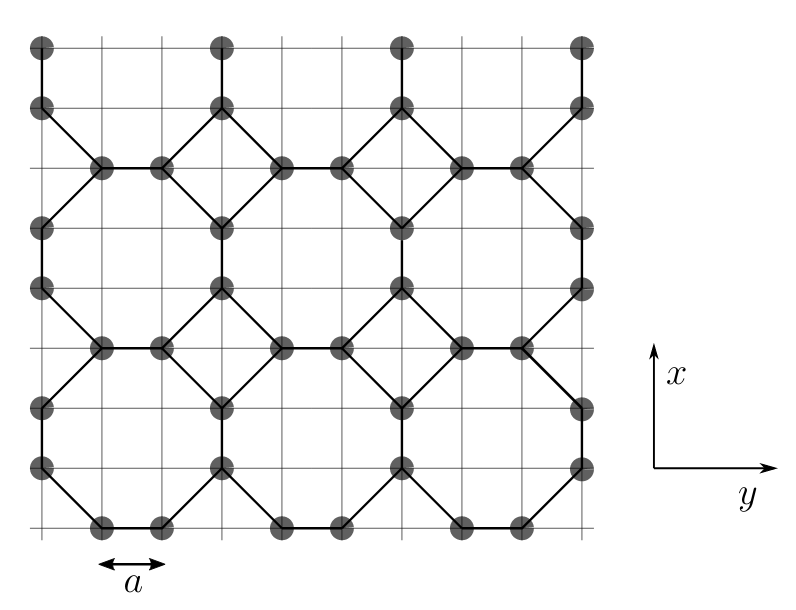
\includegraphics[width=0.5\textwidth]{./pictures/cristal2D.png}
  \caption{Cristal 2D}
  \label{fig:cristal2D}
\end{figure}

\begin{question}
  Donner les coordonnées des vecteurs $(\vv{a},\vv{b})$ qui définissent une maille primitive de ce réseau dans le repère $Oxy$ orthonormé, en fonction de $a_0$.
\end{question}

La maille est une maille carrée, les vecteurs de la maille primitive de ce réseau sont $\vv{a}=(3a,0)$ et $\vv{b}=(0,3a)$. 

\begin{question}
  Préciser la nature du réseau direct et son paramètre de maille $a$
\end{question}



\begin{question}
  Préciser le motif associé à ce cristal : nombre d'atomes et position en fonction des vecteurs $\vv{a}$ et $\vv{b}$
\end{question}


\begin{question}
  Calculer l'aire de la maille unitaire, en fonction de $a_0$
\end{question}

\begin{question}
  Calculer le nombre d'atomes par unité de surface. Application numérique en \si{\squared\meter}.
  \end{question}

\begin{question}
  Exprimer les coordonnées des vecteurs du réseau réciproque $(\vv{a*}, \vv{b*})$, en fonction de $a_0$ dans le repère $Oxy$
\end{question}


\begin{question}
  Dessiner le réseau réciproque et le première zone de Brillouin
\end{question}
\begin{question}
  Dans la première zone de Brillouin, placer les points $\Gamma$ ,$X$ de coordonnées $(\pi/a,0)$ et $M$ de coordonnées $(\pi/a,\pi/a)$.
  \end{question}





\end{document}

% LocalWords:  Hermitiques Schrödinger Hermitique
